% !TeX spellcheck = en_EN-English
\documentclass[a4paper]{article}
\usepackage[english]{babel}
\usepackage[utf8]{inputenc}
\usepackage[T1]{fontenc}
\usepackage{a4wide}
\usepackage{amsmath}
\usepackage{amsfonts}
\usepackage{amssymb}
\usepackage{mathrsfs}
\usepackage[small,bf]{caption}
\usepackage{subcaption}
\usepackage{xcolor}
\usepackage{graphicx}
\usepackage{enumerate}
\usepackage{hyperref}
\usepackage{tikz}

\let\origfontsize\fontsize
\def\fontsize#1#2{\origfontsize{11}{14.5}}

\xdef\mypath{C:/Users/majko/Desktop/weather_prediction/images}

\pagestyle{empty}
\setlength{\parindent}{0pt}

\newenvironment{modenumerate}
{\enumerate\setupmodenumerate}
{\endenumerate}

\newif\ifmoditem
\newcommand{\setupmodenumerate}{%
	\global\moditemfalse
	\let\origmakelabel\makelabel
	\def\moditem##1{\global\moditemtrue\def\mesymbol{##1}\item}%
	\def\makelabel##1{%
		\origmakelabel{##1\ifmoditem\rlap{\mesymbol}\fi\enspace}%
		\global\moditemfalse}%
}

\renewcommand{\thesubsection}{\alph{subsection})}

\makeatletter
\def\@seccntformat#1{%
	\expandafter\ifx\csname c@#1\endcsname\c@section\else
	\csname the#1\endcsname\quad
	\fi}
\makeatother
\def\checkmark{\tikz\fill[scale=0.4](0,.35) -- (.25,0) -- (1,.7) -- (.25,.15) -- cycle;} 
\begin{document} 
	
	\pagenumbering{arabic}
	\pagestyle{plain}
	
	\begin{center}
		\sc\large
		ML Project
		\\
		Determining whether weather is good for picnic 
	\end{center}
	
	Author: Marián Kravec
	
	\section{Introduction}
	
	In this project, our objective is to develop models capable of accurately assessing whether particular weather conditions, such as temperature or humidity, are conducive to an enjoyable picnic experience.
	\\
	
	Our primary aim does not involve exhaustively testing numerous models, optimizing their parameters, and identifying a singular best model. Instead, our focus is directed towards more intriguing pursuits, such as comparing the outcomes of analogous models or experimenting with techniques designed to enhance overall model performance.
	\\
	
	The project will unfold in three main segments, excluding the section introducing the data. Initially, we will undertake a comparative analysis of three implementations of the Support Vector Machine, specifically the Support Vector Classifier. This comparison will primarily involve default parameters, allowing us to identify the most effective classifier for our weather data.
	\\
	
	In the second phase, our focus will shift to Neural Networks, with a specific emphasis on transfer learning. Our objective is to explore whether incorporating transfer learning techniques contributes to enhancing the performance of our model.
	\\
	
	The concluding part centers around unsupervised learning. In this stage, we will experiment with various clustering algorithms to discern if any of them exhibit a similar data partitioning as the labeled picnic weather categories.
	
	\newpage

	\section{Data}
	
	\subsection{Source and content}
	Data used for classification and prediction are from Kaggle (\url{https://www.kaggle.com/datasets/sujaykapadnis/whether-prediction-dataset?select=weather_prediction_dataset.csv}).
	\\
	
	Dataset contains weather information from 18 different European cities (or places) measured between years 2000 and 2010 (3654 rows).
	\\
	
	Not all cities contains same set of attributes. Here is table of available attributes of each of the cities:
	
	
	\begin{table}[!h]
		\scalebox{0.7}{
		\begin{tabular}{|p{0.12\textwidth}|p{0.055\textwidth}|p{0.06\textwidth}|p{0.05\textwidth}|p{0.09\textwidth}|p{0.08\textwidth}|p{0.095\textwidth}|p{0.13\textwidth}|p{0.085\textwidth}|p{0.06\textwidth}|p{0.06\textwidth}|p{0.06\textwidth}|p{0.09\textwidth}|}
			\hline
			&  cloud cover & wind speed & wind gust & humidity & pressure & global radiation & precipitation & sunshine & temp mean & temp min & temp max & picnic weather \\ \hline
			De Bilt & \checkmark & \checkmark & \checkmark & \checkmark & \checkmark & \checkmark & \checkmark & \checkmark & \checkmark & \checkmark & \checkmark & \checkmark \\ \hline
			Tours &  & \checkmark &  & \checkmark & \checkmark & \checkmark & \checkmark &  & \checkmark & \checkmark & \checkmark & \checkmark \\ \hline
			Ljubljana & \checkmark & \checkmark &  &  & \checkmark & \checkmark & \checkmark & \checkmark & \checkmark & \checkmark & \checkmark & \checkmark \\ \hline
			Maastricht & \checkmark & \checkmark & \checkmark & \checkmark & \checkmark & \checkmark & \checkmark & \checkmark & \checkmark & \checkmark & \checkmark & \checkmark \\ \hline
			Muenchen & \checkmark & \checkmark & \checkmark & \checkmark & \checkmark & \checkmark & \checkmark & \checkmark & \checkmark & \checkmark & \checkmark & \checkmark \\ \hline
			Perpignan &  & \checkmark &  & \checkmark & \checkmark & \checkmark & \checkmark &  & \checkmark & \checkmark & \checkmark & \checkmark \\ \hline
			Heathrow & \checkmark &  &  & \checkmark &  & \checkmark & \checkmark & \checkmark &  & \checkmark & \checkmark & \checkmark \\ \hline
			Budapest & \checkmark &  &  & \checkmark & \checkmark & \checkmark & \checkmark & \checkmark & \checkmark & \checkmark & \checkmark & \checkmark \\ \hline
			Montelimar &  & \checkmark &  & \checkmark & \checkmark & \checkmark & \checkmark &  & \checkmark & \checkmark & \checkmark & \checkmark \\ \hline
			Dusseldorf & \checkmark & \checkmark & \checkmark & \checkmark & \checkmark & \checkmark & \checkmark & \checkmark & \checkmark & \checkmark & \checkmark & \checkmark \\ \hline
			Dresden & \checkmark & \checkmark & \checkmark & \checkmark &  & \checkmark & \checkmark & \checkmark & \checkmark & \checkmark & \checkmark & \checkmark \\ \hline
			Roma & \checkmark &  &  & \checkmark & \checkmark & \checkmark &  & \checkmark & \checkmark & \checkmark & \checkmark & \\ \hline
			Stockholm & \checkmark &  &  &  & \checkmark &  & \checkmark & \checkmark & \checkmark & \checkmark & \checkmark & \checkmark \\ \hline
			Malmo &  & \checkmark &  &  &  &  & \checkmark &  & \checkmark & \checkmark & \checkmark & \checkmark \\ \hline
			Sonnblick & \checkmark &  &  & \checkmark &  & \checkmark & \checkmark & \checkmark & \checkmark & \checkmark & \checkmark & \checkmark \\ \hline
			Basel & \checkmark &  &  & \checkmark & \checkmark & \checkmark & \checkmark & \checkmark & \checkmark & \checkmark & \checkmark & \checkmark \\ \hline
			Kassel &  & \checkmark & \checkmark & \checkmark & \checkmark & \checkmark & \checkmark & \checkmark & \checkmark & \checkmark & \checkmark & \checkmark \\ \hline
			Oslo & \checkmark & \checkmark & \checkmark & \checkmark & \checkmark & \checkmark & \checkmark & \checkmark & \checkmark & \checkmark & \checkmark & \checkmark \\ \hline
		\end{tabular}
		}
	\end{table}

	We will not use data for all cities, but for each part of project we will use data from different cities.

	\subsection{Data preparation}
	
	The initial step involves preparing the data in a suitable format for our models. We partition the data into city-specific datasets.
	\\
	
	During the data preparation phase for modeling, we load the data for the specified city (or cities) and randomize the order of rows. Subsequently, we divide the data into variables and labels (column-wise) and further segment it into training, testing, and validation sets (row-wise). For the training data, we calculate the average and variance of each column, employing these values to normalize all three datasets.
	\\
	
	This meticulous process ensures that the data is organized and preprocessed appropriately for subsequent model training and evaluation.
	
	\newpage

	\section{SVC comparison}
	
	Our focus is on classifying whether the weather in Basel is suitable for a picnic, utilizing a dataset with 9 attributes. To achieve this, we employ three distinct Support Vector Classifiers with slight variations. The dataset is partitioned into three segments—train, test, and validate—maintaining a ratio of 8:1:1. This division ensures an effective evaluation of the classifiers on distinct subsets of the data. 
	\\
	
	We will train these three models:
	\begin{itemize}
		\item C-Support Vector Classifier (sklearn.svm.SVC) with radial basis function kernel (we will optimize regularization parameter C)
		\item Linear Support Vector Classifier (sklearn.svm.LinearSVC) (we will optimize regularization parameter C)
		\item Linear SVC with SGD (stochastic gradient descend) training (sklearn.linear\_model.SGDClassifier with loss parameter "hinge") (we will optimize constant that multiplies the regularization term $\alpha$)
	\end{itemize}

	To assess the performance of each model, we will utilize the percentage of correctly assigned labels as the scoring metric. Enhancing the informativeness of this value, we incorporate cross-validation. The final score for each model will be derived from the average score across a 5-fold cross-validation. This approach provides a robust evaluation, capturing the model's consistency and effectiveness across different subsets of the data.
	\\
	
	After training (and optimizing chosen parameters) we get these test scores:
	
		\begin{table}[!h]
			\begin{tabular}{|l|l|l|l|}
				\hline
				model & optimized parameter & parameter value & test score  \\ \hline
				RBF kernel SVC & C & 23 & 0.89315 \\ \hline
				Linear SVC & C & 23 & 0.94247 \\ \hline
				Linear SVC with SGD& $\alpha$ & $10^{-8}$ & 0.89315 \\ \hline
			\end{tabular}
	\end{table} 

	The Linear SVC appears to outperform the other two models, which exhibit similar effectiveness. However, caution is warranted due to Goodhart's Law, emphasizing that a test score, especially when used to choose parameters, may not be a reliable measure. That's why we will compute also validation score of each model.
	\\
	
	Validation score for each of these models:
	
	\begin{table}[!h]
		\begin{tabular}{|l|l|}
			\hline
			model &  validation score  \\ \hline
			RBF kernel SVC & 0.92632 \\ \hline
			Linear SVC & 0.95361 \\ \hline
			Linear SVC with SGD &  0.88804 \\ \hline
		\end{tabular}
	\end{table} 

	
	Observing that the Linear SVC maintains the best score, it can be regarded as the top-performing model among the three. Additionally, the validation score suggests that the SVC with RBF kernel may outperform the Linear SVC with SGD. 
	\\
	
	Let's conduct the same test in two additional cities, examining different sets of attributes to compare the model rankings based on scores across datasets that are similar but have slight variations. Specifically, we will perform this test in Stockholm, which comprises only 7 attributes, and Kassel, which features 10 attributes. Notably, Kassel includes information about wind, a factor absent in the other two cities.
	\\
	
	For Stockholm we get these results:
	\begin{table}[!h]
		\begin{tabular}{|l|l|l|l|l|}
			\hline
			model & optim. parameter & parameter value & test score & validation score \\ \hline
			RBF kernel SVC & C & 11 & 0.95890 & 0.93188 \\ \hline
			Linear SVC & C & 15 & 0.98082 & 0.93995 \\ \hline
			Linear SVC with SGD& $\alpha$ & 0.2 & 0.92329 & 0.89067 \\ \hline
		\end{tabular}
	\end{table} 

	And for Kessel these:
	\begin{table}[!h]
		\begin{tabular}{|l|l|l|l|l|}
			\hline
			model & optim. parameter & parameter value & test score & validation score \\ \hline
			RBF kernel SVC & C & 7 & 0.91233 & 0.95080 \\ \hline
			Linear SVC & C & 9 & 0.95616 & 0.95905 \\ \hline
			Linear SVC with SGD& $\alpha$ & 0.5 & 0.90411 & 0.90437 \\ \hline
		\end{tabular}
	\end{table} 
	 
	The ultimate results for these two cities closely mirror those obtained for Basel, with the Linear SVC outperforming the SVC with an RBF kernel, and the linear SVC with SGD trailing in last place. Nevertheless, it's worth noting that in these two instances, the variance in validation scores between the linear kernel and RBF is negligible. Consequently, we can deem these two models equally effective in this context.
	
	\newpage

	\section{Basic neural network versus transfer learning}
	
	We have 5 cities for which we have all 12 columns, those cities are: De Bilt, Maastrich, Muenchen, Dusseldorf, Oslo. What we will try to do is train standard sequential neural network to classify whether weather in Maastrich is good for picnic. 
	\\
	
	We will compare two neural network. First NN will be trained solely using data from Masstrich. Second will be firstly trained on data from four other cities then all layers except last one will be frozen and last layer would be retrained using Masstrich data. We will then compare those two networks.  
	\\
	
	We tried multiple neural networks with different number of layers and different number of neurons in each layer and finally we ended sequential neural network with four dense layers. First three of these use hyperbolic tangent as activation function and have 24, 8 and 12 neurons respectively. Last layer use softmax as activation function and contain 2 neurons representing true and false values of our labels.    
	\\
	
	Now we can take look at accuracy of our three models (we consider model we pre-trained to use for transfer learning as third model). In this case test accuracy is computed during training by Keras library itself using 10\% of provided data which means that test accuracy of model used as pre-trained model is not accuracy on Masstrich data but accuracy on provided data from four other cities.
	
	
	\begin{figure}[h!]
		\centerline{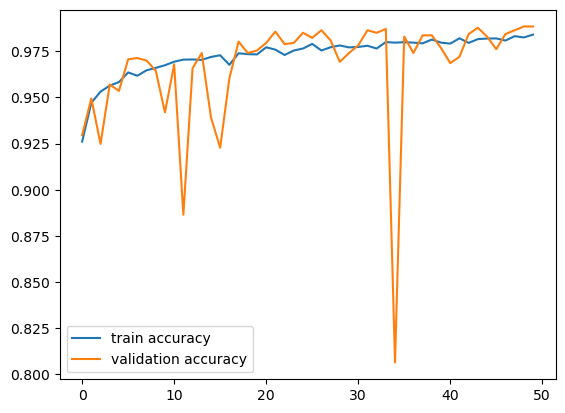
\includegraphics[width=0.85\textwidth]{\mypath/accuracy_pretrain.png}}
		\caption{Accuracy of model used for transfer learning during training}
	\end{figure}

	\begin{figure}[h!]
		\centerline{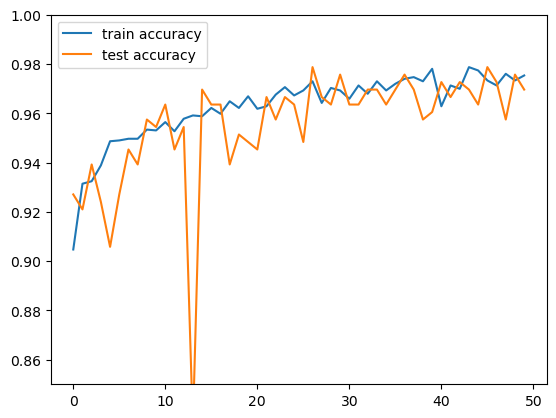
\includegraphics[width=0.85\textwidth]{\mypath/accuracy_basic.png}}
		\caption{Accuracy of model trained using only Masstrich data}
	\end{figure}

	\begin{figure}[h!]
		\centerline{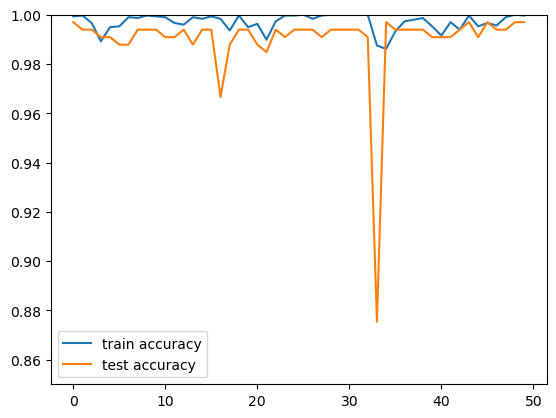
\includegraphics[width=0.85\textwidth]{\mypath/accuracy_transfer.png}}
		\caption{Accuracy of model trained using Masstrich data and pre-trained model}
	\end{figure}

	When we look at plots of accuracy of our models we can that both model that we later used as pre-trained model and model using only Maastrich steadily increased accuracy during whole training, however accuracy of model used as pre-trained is generally higher most likely thanks to bigger training dataset (approximately 4 times bigger). When we look at plot for model that is training just last layer using Maastrich data and using other layers from pre-trained model we can see that accuracy is high during whole training and improvement seems to be negligible.   
	\\
	
	If we compute validation accuracy using approximately 10\% of Maastrich data not used during training we get these values for our three models:
	\begin{table}[!h]
		\begin{tabular}{|l|l|}
			\hline
			model &  validation accuracy  \\ \hline
			Pre-trained on different cities  & 0.98356 \\ \hline
			Standard Neural Network & 0.97260 \\ \hline
			Trasfer learning using pre-trained &  0.99178 \\ \hline
		\end{tabular}
	\end{table} 

	We can see that model that was used as pre-trained model acquire slightly better result than standard model even though it has disadvantage that it never saw any data from Maastrich. Our model that used transfer learning from pre-trained model acquired highest accuracy which would imply that transfer learning really improved model. However because differences between accuracy of these model is very small it is not appropriate to draw any conclusion.
	
	
	\section{Unsupervised learning - clustering}
	
	We will use four different models with mostly default setting as we are consider it to be unsupervised learning so we don't use labels to improve model but just validate it.
	\\
	
	Here are model we will compare:
	\begin{itemize}
		\item K-Means Clustering (sklearn.cluster.KMeans) - standard Kmeans using Lloyd's algorithm, that is trying to minimize sum of distances between point and center of cluster point belong to
		\item Spectral Clustering (sklearn.cluster.SpectralClustering) - that compute affinity matrix of points using RBF kernel, then compute Laplacian matrix from it and finally compute clusters using K-Means algorithm on Laplacian projection of points
		\item Agglomerative Clustering (sklearn.cluster.AgglomerativeClustering) - hierarchical clustering algorithm that recursively merges pair of clusters of sample data minimizing the variance of the clusters being merged
		\item Gaussian Mixture (sklearn.mixture.GaussianMixture) - this model is trying to represent each sample data as point generated by one of multiple Gaussian distribution, initial it split points using K-Means algorithm and then optimize their affiliation to Gaussian distributions using EM algorithm
	\end{itemize}

	We will try this algorithm on data from three different cities Budapest, Perpignan and Dresden. Validation score is computed as percentage of correctly "labeled" validation data point (mapping between clusters and labels values is such that maximize validation score which means that minimal score is 0.5). We will also compare our models to base model which put all points into one cluster so assume that all data has same label (majority one). (we can also consider one more base model splitting points into clusters randomly but that model would always have minimal possible score 0.5 because of a away we map clusters to labels)
	\\
	
	Now let's look at results for each of our three cities:
	\\
	
	Budapest:
	\begin{table}[!h]
		\begin{tabular}{|l|l|}
			\hline
			model &  validation score  \\ \hline
			Base & 0.62466 \\ \hline
			K-Means Clustering & 0.89863 \\ \hline
			Spectral Clustering &  0.89315 \\ \hline
			Agglomerative Clustering  &  0.85479 \\ \hline
			Gaussian Mixture &  0.90137 \\ \hline
		\end{tabular}
	\end{table} 

	We can see that compared to base model all our models seems to have significantly higher score. Except Agglomerative Clustering all models has score around 0.9 which means 90\% accuracy. Based on this we can conclude that all our models split data into clusters similar to their labeling.
	\\
	
	Perpignan:
	\begin{table}[!h]
		\begin{tabular}{|l|l|}
			\hline
			model &  validation score  \\ \hline
			Base & 0.53150 \\ \hline
			K-Means Clustering & 0.83836 \\ \hline
			Spectral Clustering &  0.51232 \\ \hline
			Agglomerative Clustering  &  0.79726 \\ \hline
			Gaussian Mixture &  0.82192 \\ \hline
		\end{tabular}
	\end{table} 

	Here we see that base model has score barely over 0.5 which implies that our validation dataset contains approximately same number of each label. When we take a look at scores of our model we can see that three models significantly outperformed base model, while Spectral Clustering got score close to minimal possible, so their is most likely no relationship between this split and labels.
	\\

	Dresden:
	\begin{table}[!h]
		\begin{tabular}{|l|l|}
			\hline
			model &  validation score  \\ \hline
			Base & 0.77808 \\ \hline
			K-Means Clustering & 0.77534 \\ \hline
			Spectral Clustering &  0.77260 \\ \hline
			Agglomerative Clustering  &  0.73424 \\ \hline
			Gaussian Mixture &  0.80822 \\ \hline
		\end{tabular}
	\end{table} 
	
	Here we can see that base model has score around 0.77 which means that validation data for this city is quite skewed towards one label value. Here we can see that all our models acquired score close to base model score so we can't conclude any model do be significantly better then base model.
	\\
	
	In general it seems that for data such as our best model to determine whether weather is good for picnic without need to label data is Gaussian Mixture model which for all three cities ended as either best or second to best model. However if data is highly skewed towards one label even this model might not be useful.
	\\
	
	Now we will visualize our best and our worst result. To do it we reduce our data into two dimensional data using PCA algorithm and then visualize out data using scatter plot with labels (clusters) as colors of points.
	\\
	
	So our best model was Gaussian Mixture model for Budapest data:
	
	\begin{figure}[h!]
		\centerline{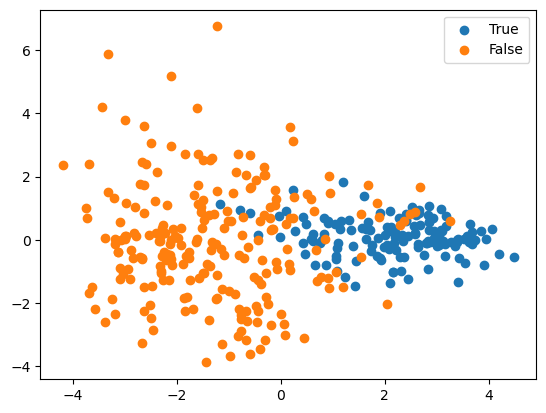
\includegraphics[width=0.85\textwidth]{\mypath/budapest_label.png}}
		\caption{Real split into weather suitable and not suitable for picnic in Budapest}
	\end{figure}
	
	\begin{figure}[h!]
		\centerline{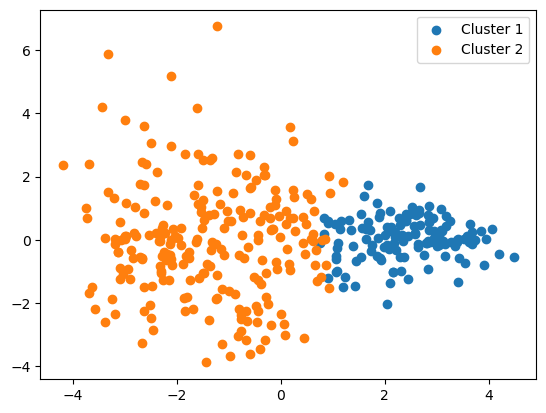
\includegraphics[width=0.85\textwidth]{\mypath/budapest_gauss.png}}
		\caption{Split into weather suitable and not suitable for picnic in Budapest using Gaussian Mixture model}
	\end{figure}

	We can clearly see resemblance between those two splits, we can also see that even though we reduced dimension using PCA we can still clearly see border between clusters in Gaussian Mixture model, but border between real labels is much more vague.
	\\
	
	Our worst performing model was Spectral Clustering for Perpignan data that has score similar to either one cluster or random model.
	
	\begin{figure}[h!]
		\centerline{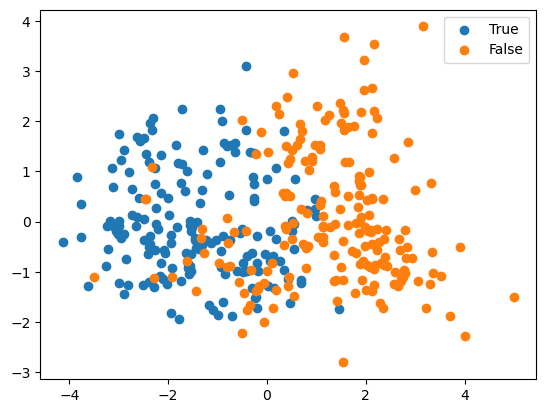
\includegraphics[width=0.85\textwidth]{\mypath/perpignan_label.png}}
		\caption{Real split into weather suitable and not suitable for picnic in Perpignan}
	\end{figure}
	
	\begin{figure}[h!]
		\centerline{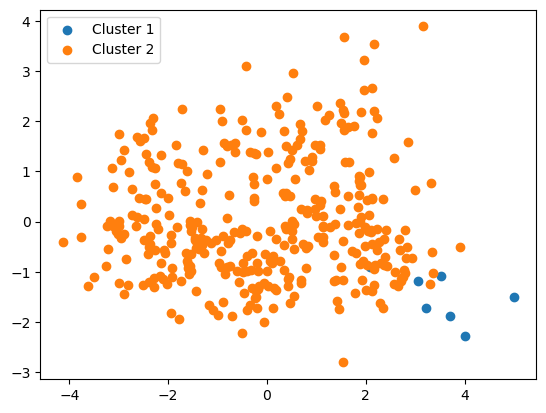
\includegraphics[width=0.85\textwidth]{\mypath/perpignan_spectral.png}}
		\caption{Split into weather suitable and not suitable for picnic in Perpignan using Spectral Clustering model}
	\end{figure}
	
	Here we clearly see why Spectral Clustering model is so close base model with one cluster as it formed one big cluster containing more than 98\% of data points. If we take a look at real labeling we see vague border between label groups but as we saw based on results from other models approximation of this border is to some extend achievable without knowledge of labels.
	
\end{document}